\documentclass{article}
\usepackage[left=0.5in,top=0.5in,right=0.5in,bottom=0.5in]{geometry}
\usepackage[english]{babel}
\usepackage[utf8]{inputenc}
\usepackage[table]{xcolor}
\usepackage{amssymb,amsmath,amsthm}
\usepackage{changepage,threeparttable}
\usepackage{booktabs,multirow}
\usepackage{graphicx}
\usepackage{soul}
\graphicspath{{./images/}}
\def\F#1{\(#1\)}
\title{Lab 13: The DIY Inductor}
\author{Philip Kim}
\date{\today}
\begin{document}
\maketitle
\vspace*{-1cm}
\begin{table}[!htp]\centering
  \begin{tabular}{|c|c|}\hline
    \multicolumn{2}{|c|}{\textbf{Table 1: Sizes}}\\\hline
    Copper wire length l& \\\hline
    Diameter of pen d& \\\hline
    Number of windings N& \\\hline
    Length of the inductor a& \\\hline
  \end{tabular}
\end{table}
\begin{table}[!htp]\centering
  \begin{tabular}{|c|c|c|c|c|c|c|}\hline
    \multicolumn{7}{|c|}{\textbf{Table 2: First Approximation for \F{R_{int}}}}\\\hline
    \F{f (Hz)}&\F{s/DIV}&\F{V_{RL} (V)}&\F{V/DIV} for \F{V_{RL}}&\F{V_L (V)}&\F{V/DIV} for \F{V_L}&\F{R_{int} (\Omega)}\\\hline
    1000& & & & & & \\\hline
  \end{tabular}
\end{table}
\begin{table}[!htp]\centering
  \begin{tabular}{|c|c|c|c|c|c|c|c|c|c|}\hline
    \multicolumn{10}{|c|}{\textbf{Table 2: First Approximation for \F{L}}}\\\hline
    \F{f (Hz)}&\F{s/DIV}&\F{V_{RL} (V)}&\F{V/DIV} for \F{V_{RL}}&\F{V_L (V)}&\F{V/DIV} for \F{V_L}&\F{I_R (A)}&\F{Z_{L,eff} (\Omega)}&\F{X_L (\Omega)}&\F{L (H)}\\\hline
    65000& & & & & & & & & \\\hline
  \end{tabular}
\end{table}
\begin{table}[!htp]\centering
  \begin{tabular}{|c|c|c|c|c|c|}\hline
    \multicolumn{6}{|c|}{\textbf{Table 3: The Impedance of an Inductor}}\\\hline
    \F{f (Hz)}&s/DIV&\F{V_{RL} (V)}&V/DIV for \F{V_{RL}}&\F{V_{L} (V)}&V/DIV for \F{V_{L}}\\\hline
    1000& & & & & \\\hline
    22000& & & & & \\\hline
    32000& & & & & \\\hline
    39000& & & & & \\\hline
    45000& & & & & \\\hline
    50000& & & & & \\\hline
    55000& & & & & \\\hline
    60000& & & & & \\\hline
    65000& & & & & \\\hline
  \end{tabular}
\end{table}
\begin{center}
  \subsection*{Setup}
  % 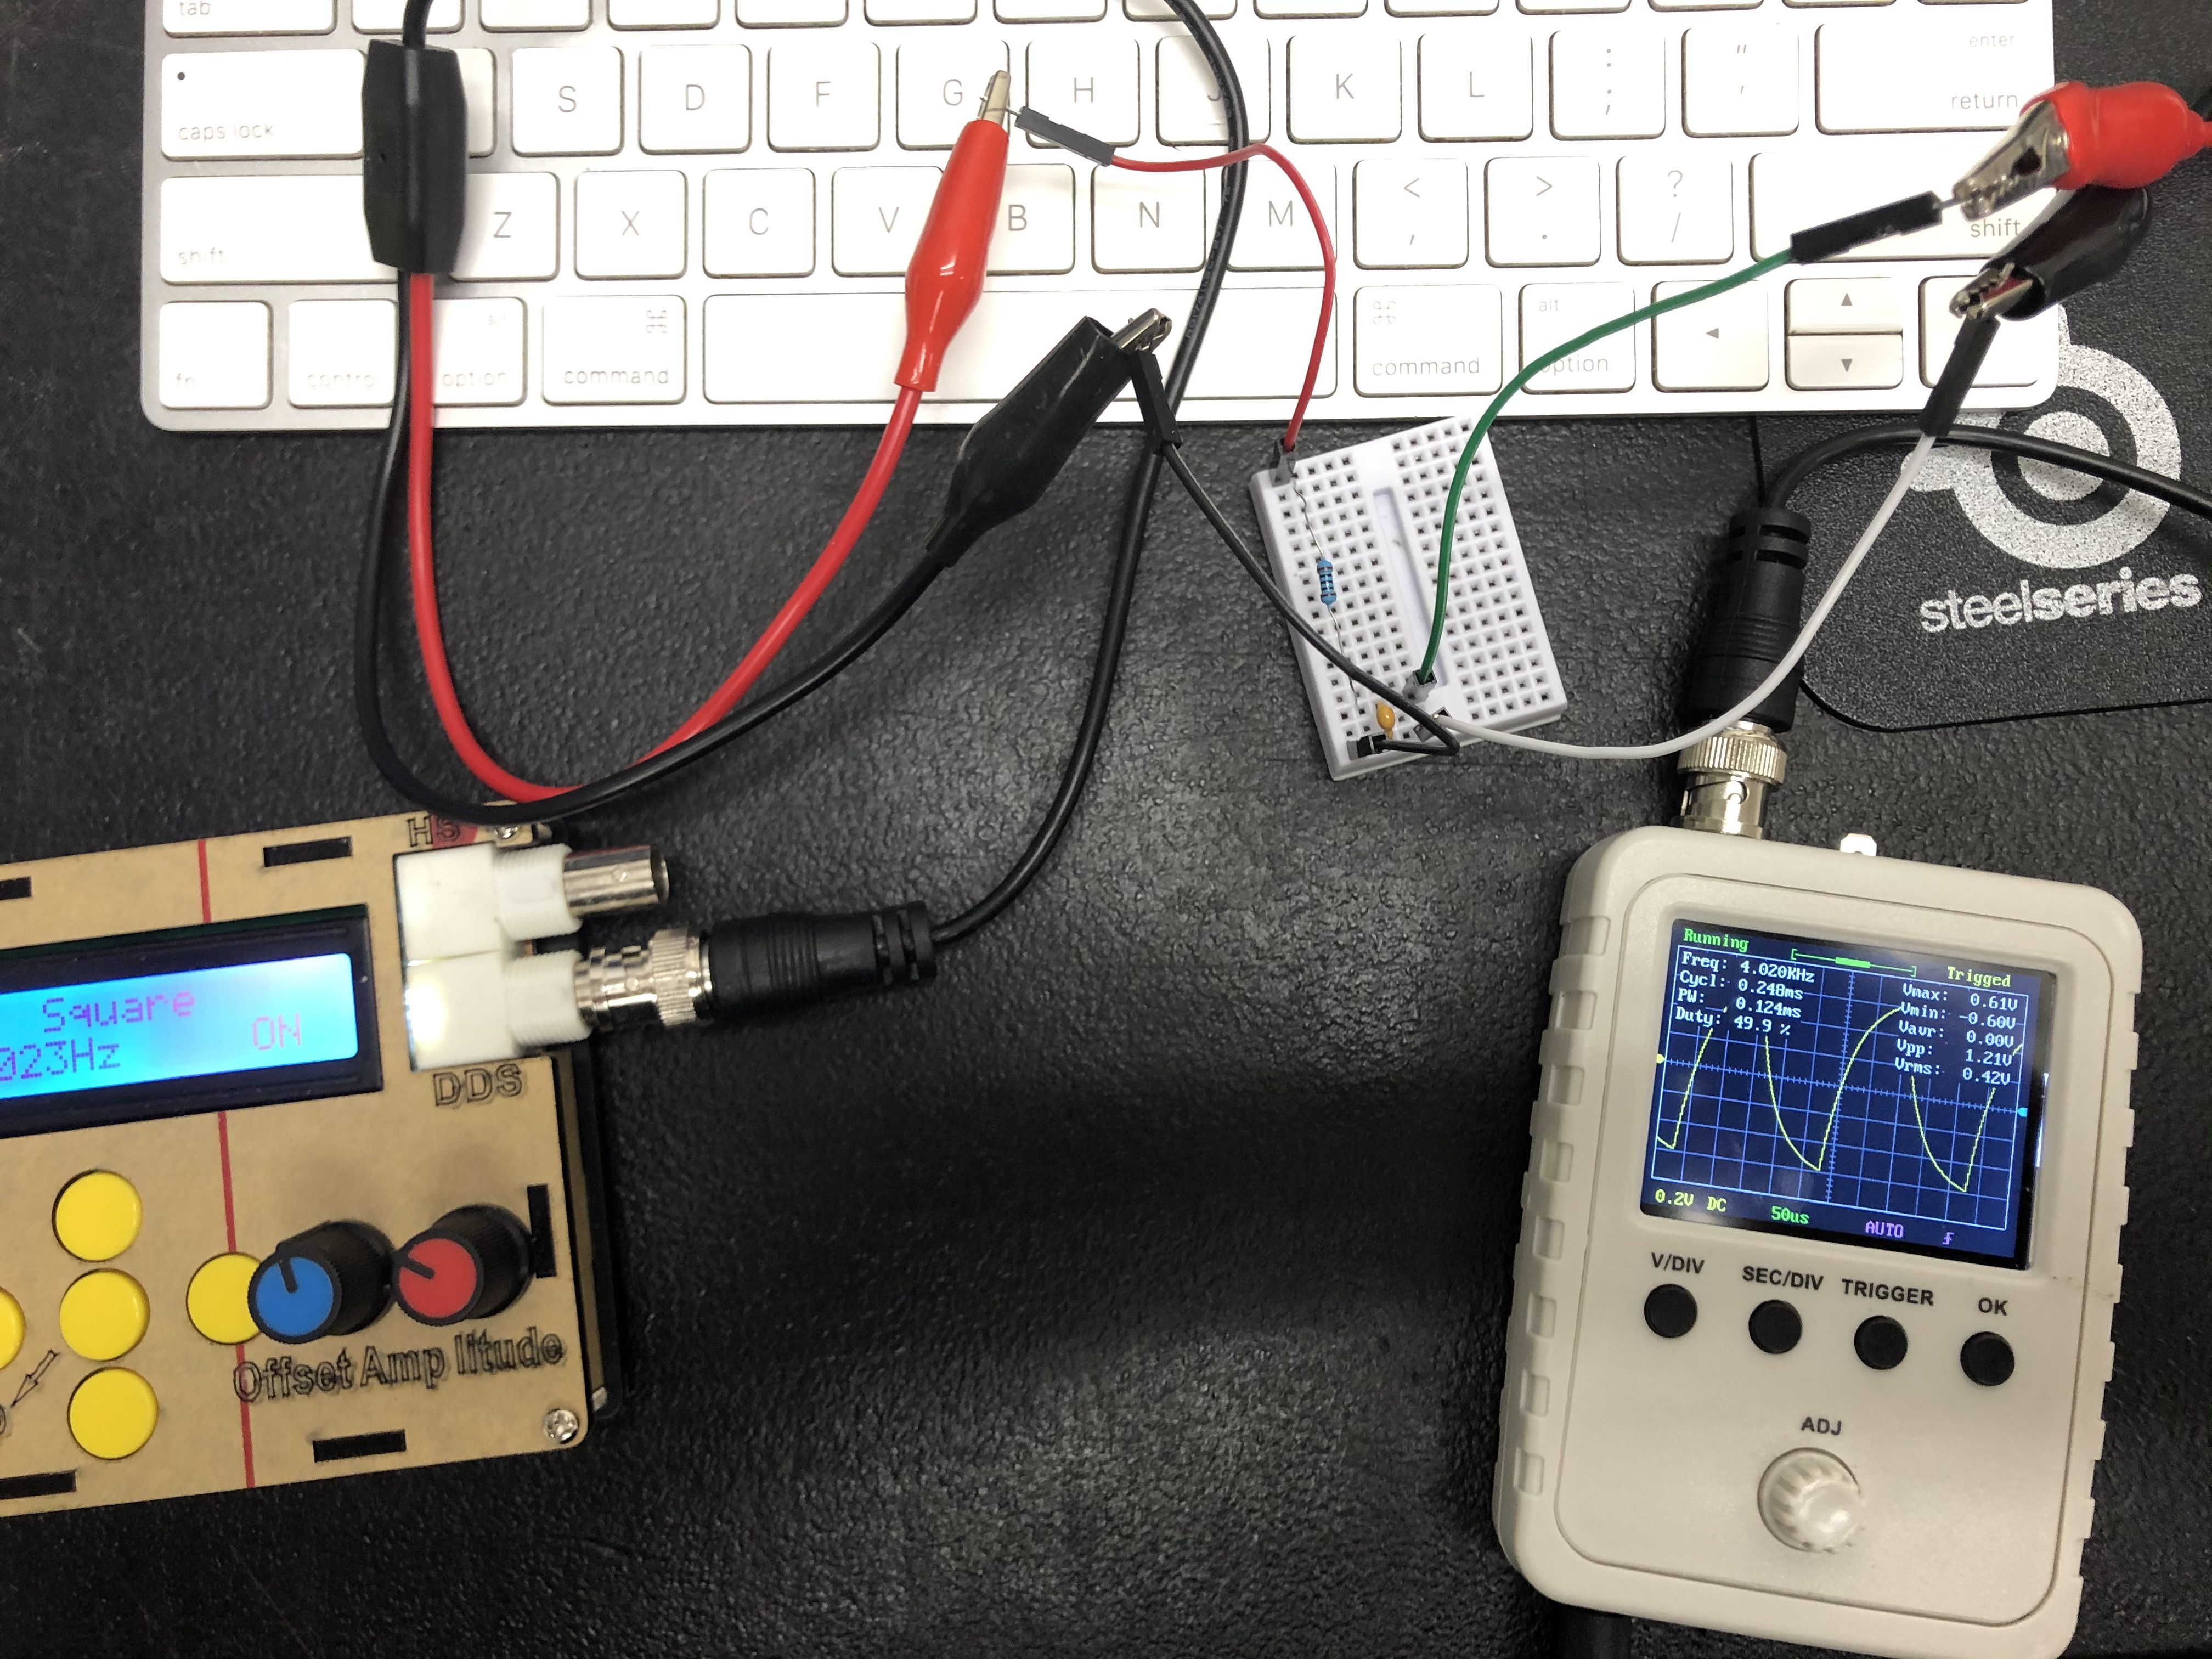
\includegraphics[scale=0.066]{setup1.jpeg}
  setup
  \subsection*{Graph 1}
  % 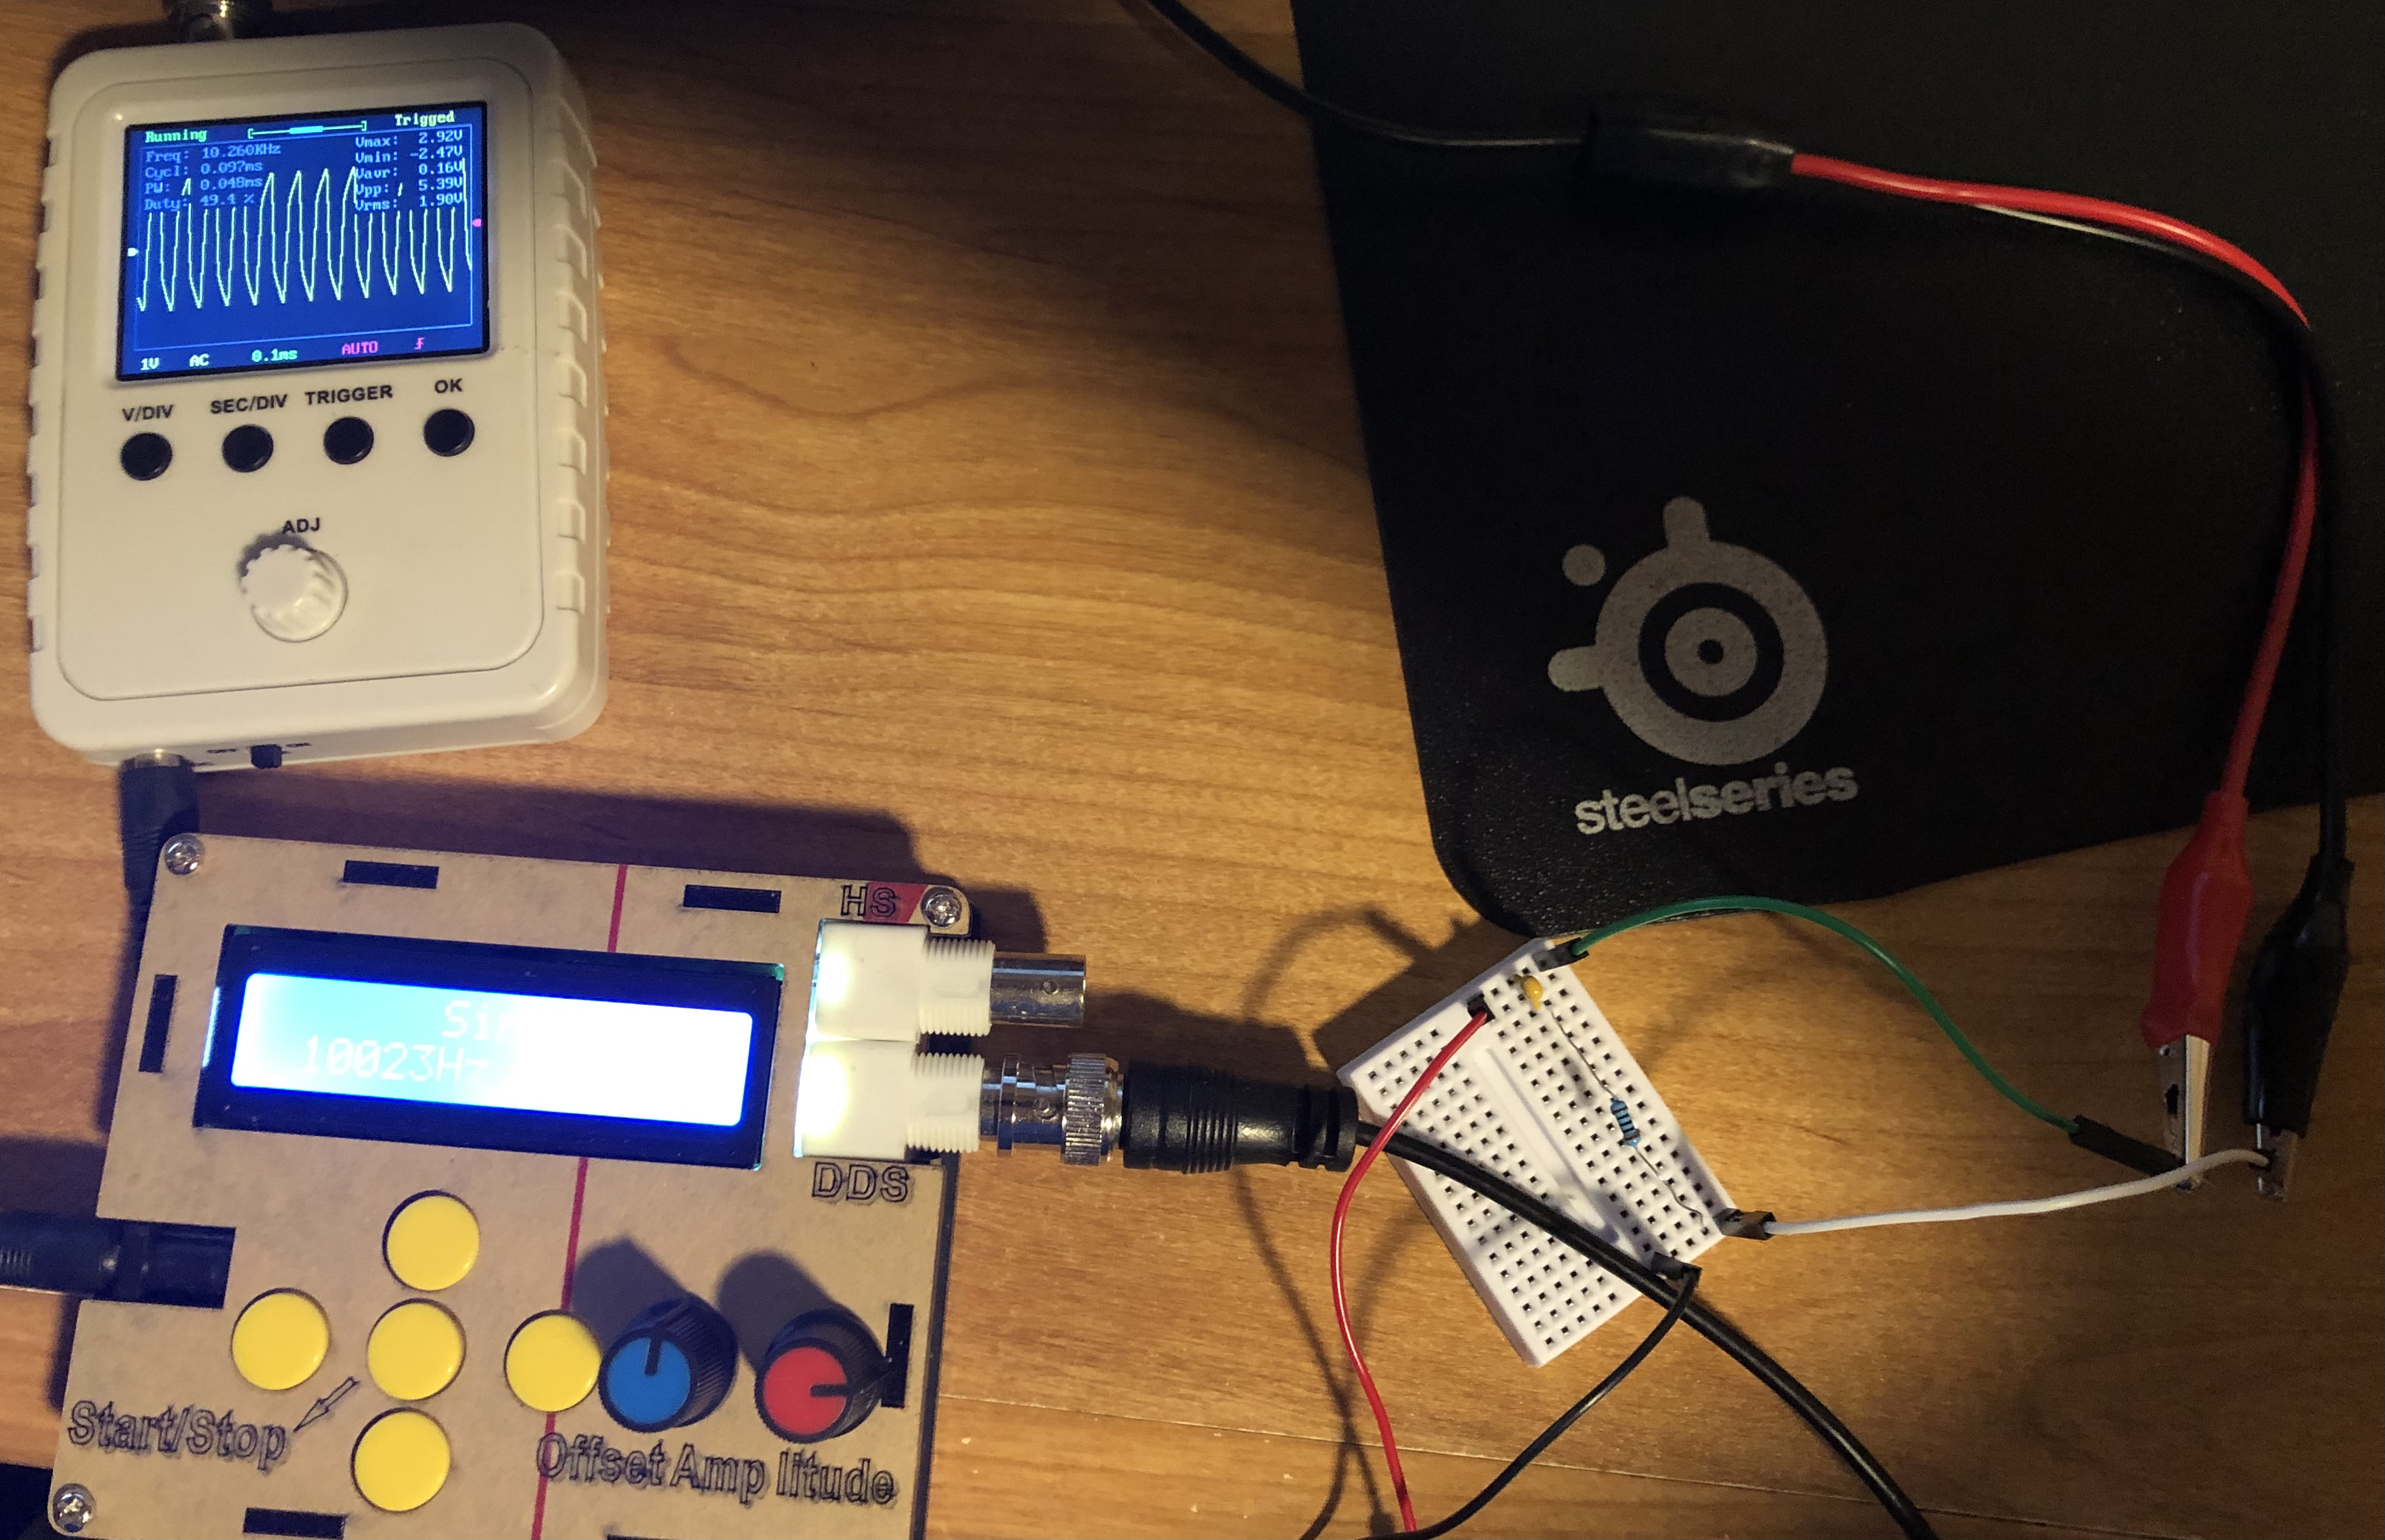
\includegraphics[scale=0.066]{Vrc.jpeg}
  graph 1
  \subsection*{Calculation}
  Calculation
\end{center}
\begin{itemize}
  \item Compare the obtained value to that predicted for an ideal long inductor made of a wire of length l and taking up length a along the toothpick, \F{L=\frac{l^2}{a}\times{10}^{-7}H}
\end{itemize}
\end{document}
